\section{Question 3}
Perform an experiment testing different kernel functions and hyperparameter configurations 
to obtain the best SVM classifier for a binary classification task, using a dataset of your choice. 
Don't forget to discuss the results.

\noindent\rule{\textwidth}{.5pt}

\noindent\textbf{Data description.}
\begin{figure}[!ht]
    \centering
    \caption{
        Feature correlations found in a subset of Parkinson Detection dataset 
        (a) before and (b) after removing highly-correlated features.
    }
    \label{fig:correlations_pd}
    \begin{subfigure}{.49\textwidth}
        \centering
        \caption{}
        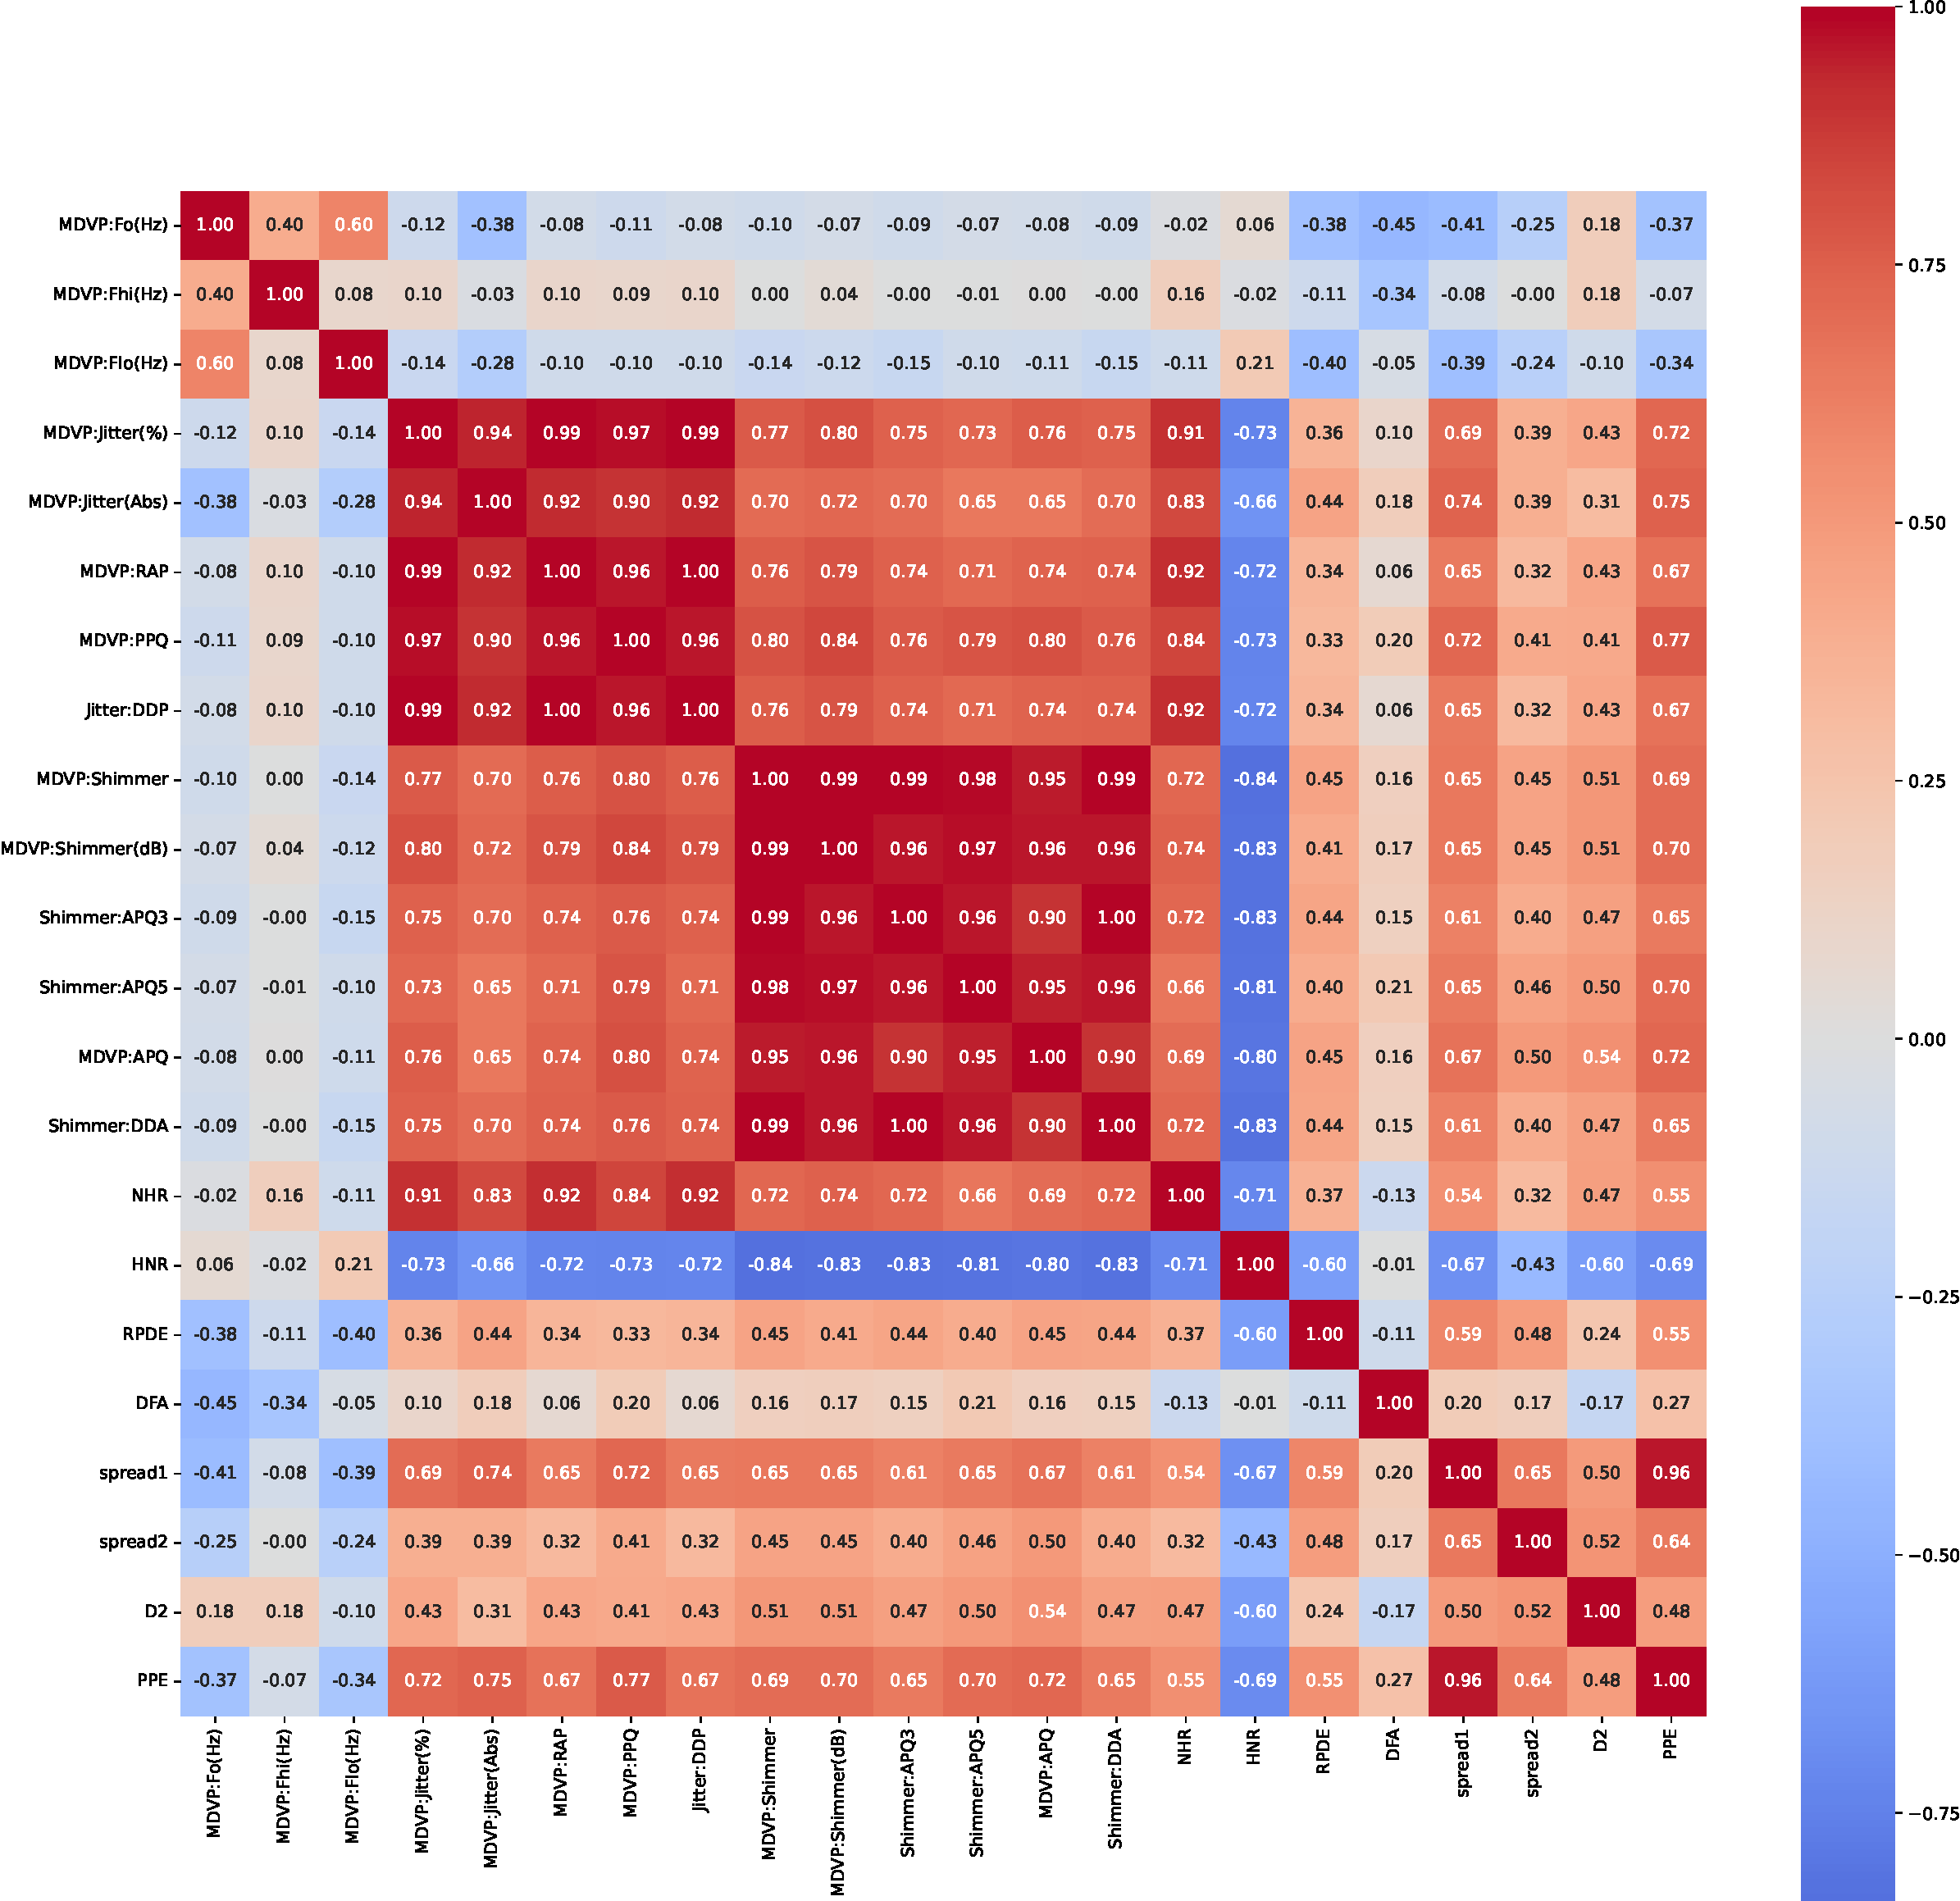
\includegraphics[width=\linewidth]{../../python_code/plots/original_correlations_parkinsons.pdf}
    \end{subfigure}
    \begin{subfigure}{.49\textwidth}
        \centering
        \caption{}
        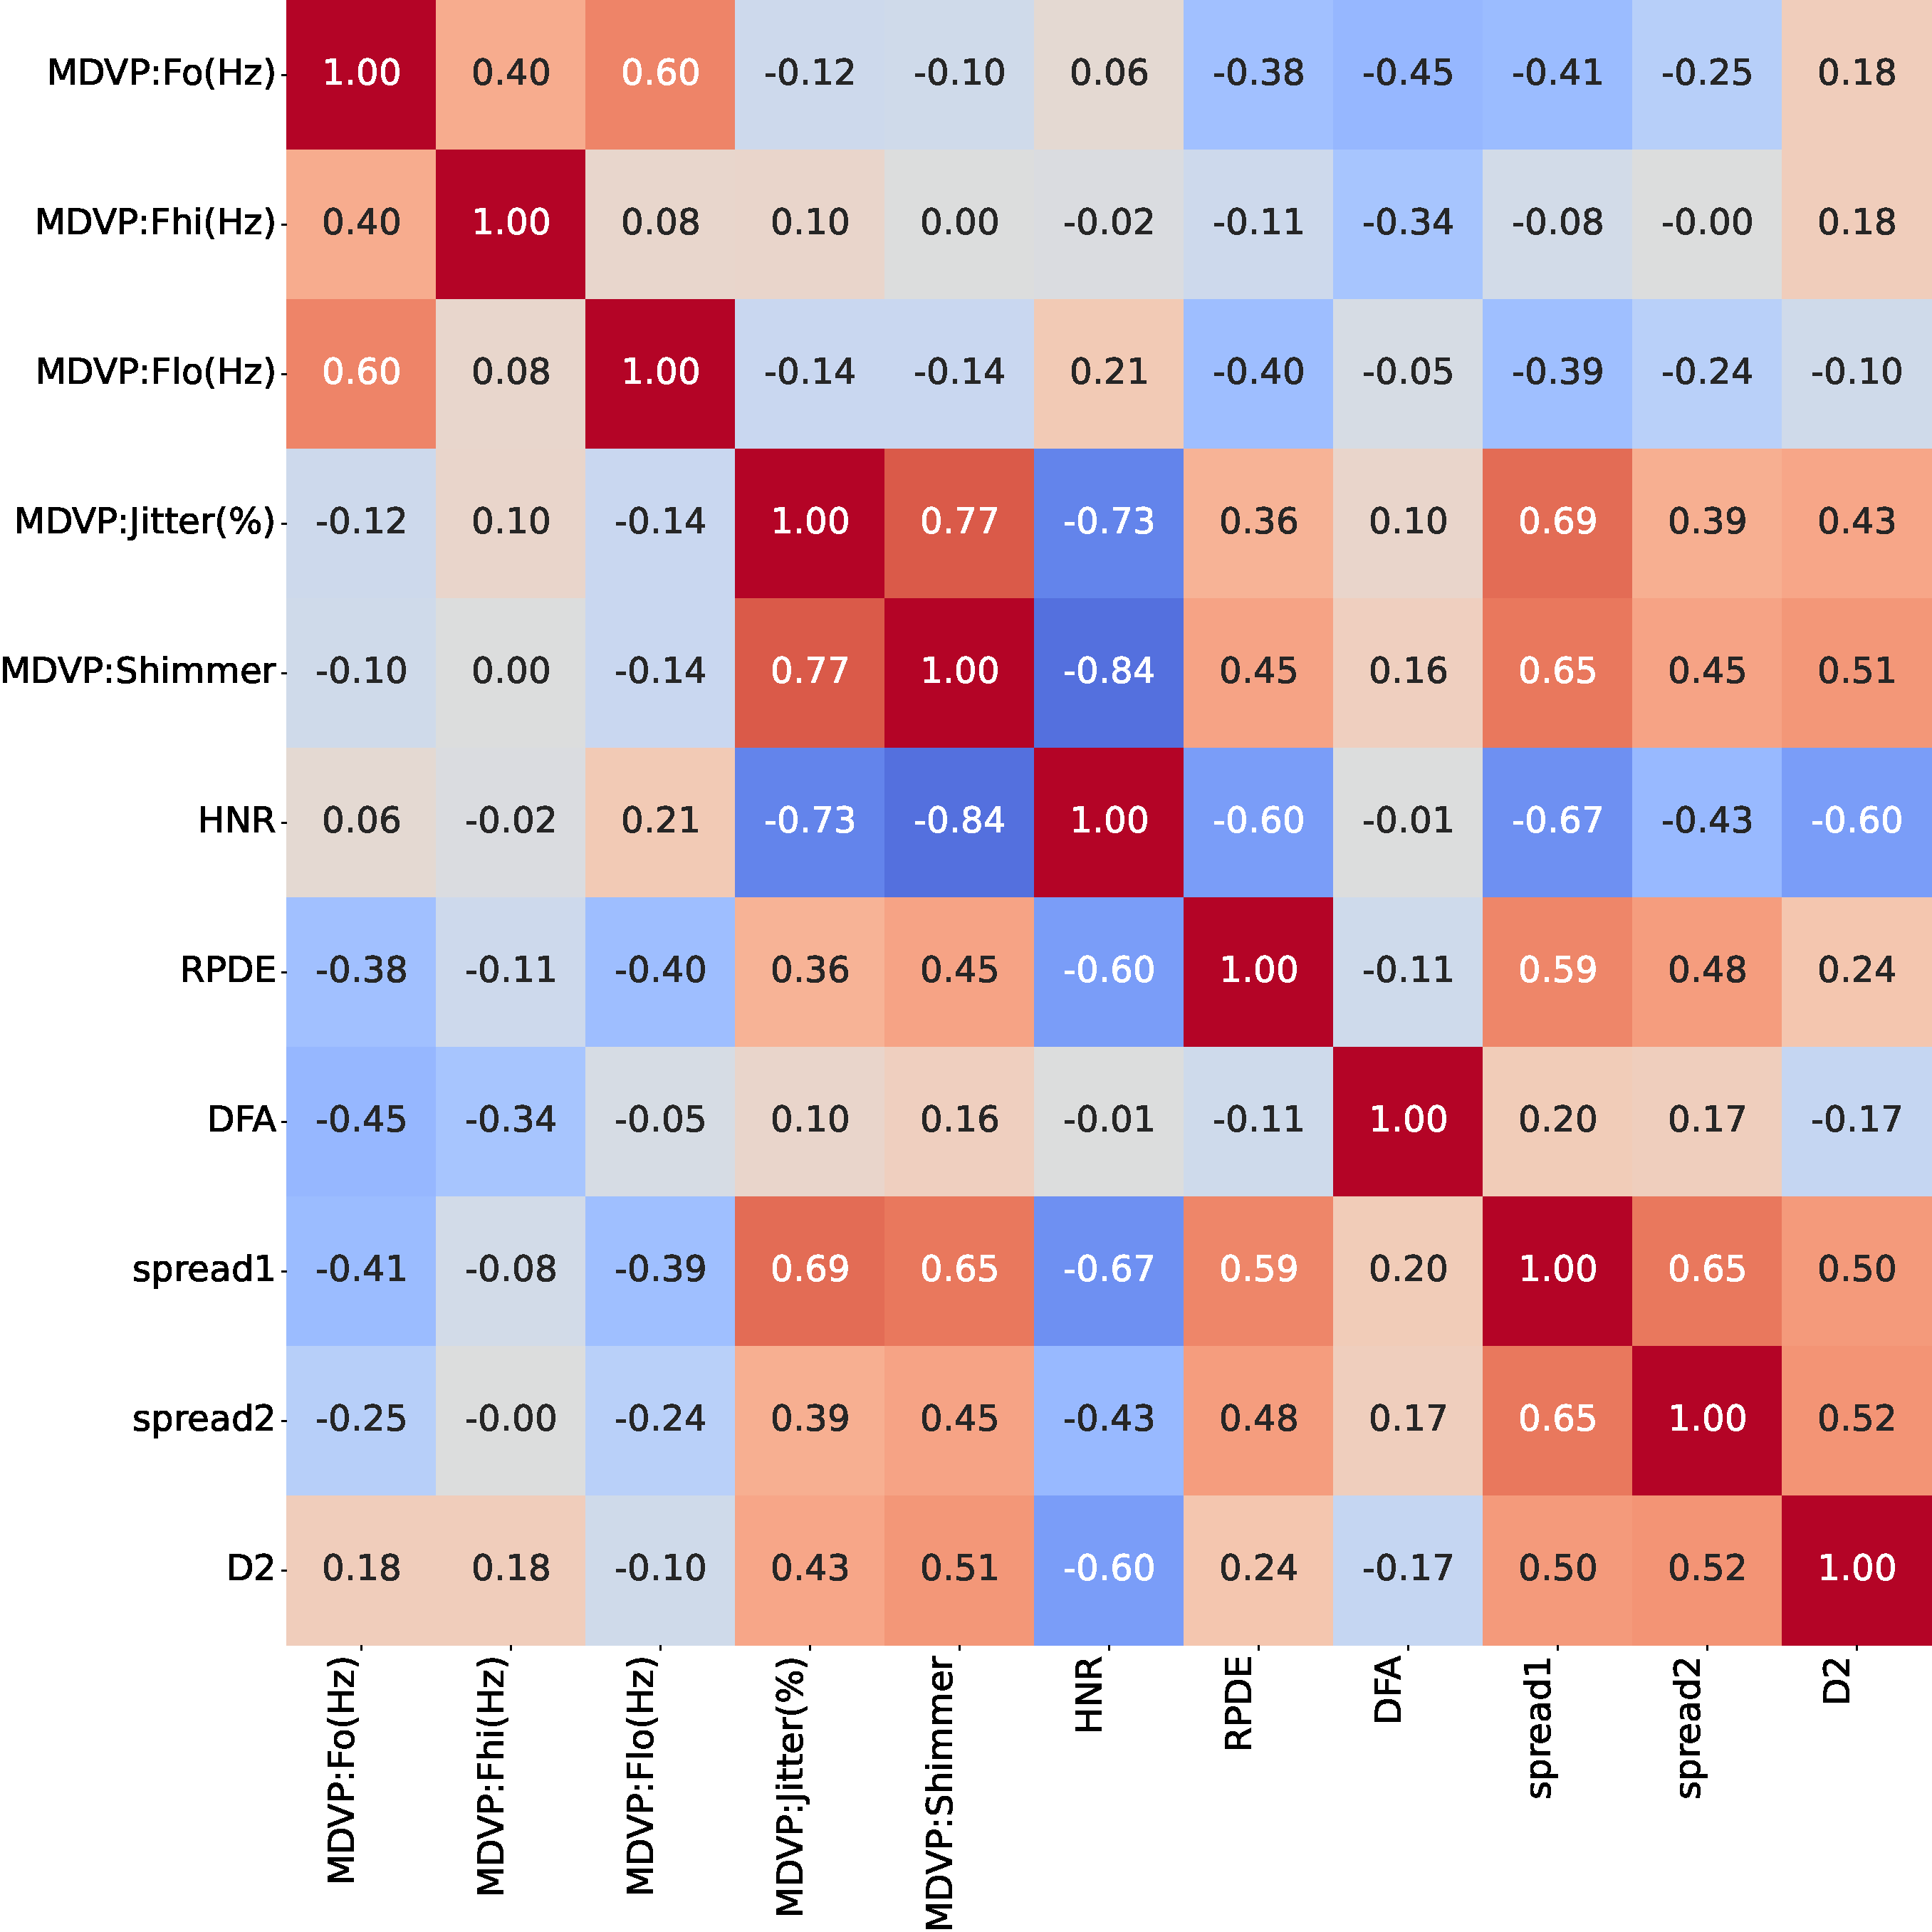
\includegraphics[width=\linewidth]{../../python_code/plots/filtered_correlations_parkinsons.pdf}
    \end{subfigure}
\end{figure}

\begin{table}[!h]
    \centering
    \begin{threeparttable}
    \caption{SVM hyperparameters.}
    \label{tab:hparams_svm}
    \begin{tabular}{ccc}
        \toprule
            Hyperparameter & Possible values & Best after 100 trials \\
        \midrule
            Kernel & Linear, polynomial, RBF$^*$ or sigmoid & RBF \\
            Regularization constant$^{**}$ & $[10^{-1}, 10^3]$ & 17.72\\
        \bottomrule
    \end{tabular}
    \begin{tablenotes}
        \item $^*$ Radial Basis Function 
        \item $^{**}$ Sampled from the log domain
    \end{tablenotes}
\end{threeparttable}
\end{table}

\begin{figure}[!ht]
    \centering
    \caption{Confusion matrix of best SVM.}
    \label{fig:confusion_matrix_svm}
    
\includegraphics[width=0.5\textwidth]{../../python_code/plots/svm/confusion_matrix.pdf}
\end{figure}